\documentclass[10pt,english,aspectratio=169]{beamer}
% Use notes or hide notes or show only notes or handout

\usetheme{default}

\usepackage{xstring}
\usepackage{pgfpages}
%\makeatletter
%\IfSubStr{\@classoptionslist}{handout}
%  {\pgfpagesuselayout{2 on 1}[letterpaper,border shrink=5mm]}
%  {}
%\makeatother

\usepackage{amsmath,amssymb,amsthm}
\usepackage{stmaryrd}
\usepackage{enumerate}
\usepackage{stfloats}
\usepackage{bbm}
\usepackage{pdfpages}
\usepackage{framed}

\usepackage[most]{tcolorbox}
\tcbset{highlight math style={enhanced,
  colframe=white,colback=yellow!15,arc=8pt,boxrule=1pt,
  }}
  
\usepackage{tikz,pgf,pgfplots}
\usepackage{algorithm,algorithmic}
\usepgflibrary{shapes}
\usetikzlibrary{%
  arrows,%
  arrows.meta,
  backgrounds,
  shapes.misc,% wg. rounded rectangle
  shapes.arrows,%
  shapes,%
  calc,%
  chains,%
  matrix,%
  positioning,% wg. " of "
  scopes,%
  decorations.pathmorphing,% /pgf/decoration/random steps | erste Graphik
  shadows,%
  backgrounds,%
  fit,%
  petri,%
  quotes
}

\tikzset{background rectangle/.style={
    fill=white,
  },
  use background/.style={    
    show background rectangle
  }
}

\setbeamersize{text margin left=10mm,text margin right=35mm}

\pgfplotsset{compat=1.12}

%\usetheme{Frankfurt}
%\usecolortheme{ldpc}
\useinnertheme{rounded}
\usecolortheme{whale}
\usecolortheme{orchid}

\newcommand{\ul}[1]{\underline{#1}}
\renewcommand{\Pr}{\mathbb{P}}

%% Setup slides and notes
\makeatletter
\IfSubStr{\@classoptionslist}{notes} { \IfSubStr{\@classoptionslist}{hide} {}{\IfSubStr{\@classoptionslist}{only} {}{\setbeameroption{show notes on second screen=right}}} }{}
\makeatother
%\setbeamertemplate{note page}{\pagecolor{yellow!5}\vfill\insertnote\vfill}

\newcommand{\getpdfpages}[2]{\begingroup
  \setbeamercolor{background canvas}{bg=}
  \addtocounter{framenumber}{1}
  \includepdf[pages={#1},%
  pagecommand={%
    \expandafter\def\expandafter\insertshorttitle\expandafter{%
      \insertshorttitle\hfill\insertframenumber\,/\,\inserttotalframenumber}}%
  ]{#2}
  \endgroup}

\newcommand{\backupbegin}{
   \newcounter{finalframe}
   \setcounter{finalframe}{\value{framenumber}}
}
\newcommand{\backupend}{
   \setcounter{framenumber}{\value{finalframe}}
}

 \setbeamercolor{bibliography entry author}{fg=black}
 \setbeamercolor{bibliography entry title}{fg=black}
 \setbeamercolor{bibliography entry location}{fg=black}
 \setbeamercolor{bibliography entry note}{fg=black}
 
 \setbeamerfont{bibliography item}{size=\footnotesize}
 \setbeamerfont{bibliography entry author}{size=\footnotesize}
 \setbeamerfont{bibliography entry title}{size=\footnotesize}
 \setbeamerfont{bibliography entry location}{size=\footnotesize}
 \setbeamerfont{bibliography entry note}{size=\footnotesize}
 \setbeamertemplate{bibliography item}{\insertbiblabel}
 
\newlength\tikzwidth
\newlength\tikzheight


\newcommand{\mc}[1]{\mathcal{#1}}
\newcommand{\mbb}[1]{\mathbb{#1}}
%\newcommand{\expt}{\mbb{E}}
%\newcommand{\dd}{\mathrm{d}}
\newcommand{\Interior}[1]{\ensuremath{{#1}^{\circ}}}
\newcommand{\Closure}[1]{\ensuremath{\overline{#1}}}
\newcommand{\Complement}[1]{\ensuremath{{#1}^{c}}}

\newcommand{\Expect}{\ensuremath{\mathrm{E}}}
\newcommand{\vecnot}{\underline}
\newcommand{\RealNumbers}{\ensuremath{\mathbb{R}}}
\newcommand{\RationalNumbers}{\mathbb{Q}}
\newcommand{\ComplexNumbers}{\mathbb{C}}
\newcommand{\Real}{\mathrm{Re}}
\newcommand{\Span}{\mathrm{span}}
\newcommand{\Rank}{\mathrm{rank}}
\newcommand{\Nullity}{\mathrm{nullity}}
\newcommand{\Trace}{\mathrm{tr}}
\newcommand{\Diag}{\mathrm{diag}}
\newcommand{\dd}{\mathrm{d}}
\DeclareMathOperator*{\esssup}{ess\,sup}

% Use < , > inner product
\newcommand{\inner}[2]{{\left\langle #1 \mskip2mu , #2 \right\rangle}}
\newcommand{\tinner}[2]{{\langle #1 \mskip1mu , #2 \rangle}}

% Use < | > inner product
%\newcommand{\inner}[2]{{\left\langle #1 \mskip2mu \middle| \mskip2mu #2 \right\rangle}}
%\newcommand{\tinner}[2]{{\langle #1 \mskip1mu | \mskip1mu  #2 \rangle}}




\def\checkmark{\tikz\fill[scale=0.4](0,.35) -- (.25,0) -- (1,.7) -- (.25,.15) -- cycle;}
\def\greencheck{{\color{green}\checkmark}}
\def\scalecheck{\resizebox{\widthof{\checkmark}*\ratio{\widthof{x}}{\widthof{\normalsize x}}}{!}{\checkmark}}
\def\xmark{\tikz [x=1.4ex,y=1.4ex,line width=.2ex, red] \draw (0,0) -- (1,1) (0,1) -- (1,0);}
\def\redx{{\color{red}\xmark}}

\renewcommand{\footnotesep}{-2pt}


\begin{document}

\title{ECE 586: Vector Space Methods \\ Lecture 11 Flip Video: Linear Transforms}
\author{Henry D. Pfister \\ Duke University}
\date{}
%\date{August 20th, 2020}
%\maketitle

\setbeamertemplate{navigation symbols}{}

\begin{frame}[plain]
	\titlepage
	
	\note{
		\vspace{8mm}
		\begin{enumerate}
			\setlength\itemsep{3mm}
			\color{red}
			\item Welcome to the 11th video lecture for ECE 586, Vector Space Methods. \\[2mm]
			Today, we'll finish our discussion of subspaces and bases and then move on to linear transforms.
		\end{enumerate}
	}
\end{frame}

\addtocounter{framenumber}{-1}
\setbeamertemplate{navigation symbols}{\textcolor{blue}{\footnotesize \insertframenumber ~/ \inserttotalframenumber}}


\begin{frame}<1-4> \frametitle{Sums and Direct Sums}

\vspace{-1mm}

\begin{definition}<1->
Let $U,W$ be subsets of a vector space $V$.
The \textcolor{blue}{sum} of $U$ and $W$ is defined by \vspace{-2mm}
\begin{equation*}
U + W \triangleq \left\{ \vecnot{v} \in V \, \middle| \, \exists \vecnot{u} \in U, \exists \vecnot{w} \in W, \vecnot{v} = \vecnot{u} + \vecnot{w} \right\}.
\end{equation*}
\end{definition}

\begin{definition}<2->
For a vector space $V$, subspaces $U$ and $W$ are called \textcolor{blue}{disjoint} if $U \cap W = \{\vecnot{0}\}$.
\end{definition}

\begin{definition}<3->
For disjoint subspaces $U$ and $W$ in a vector space, their \textcolor{blue}{direct sum}  equals their sum but is denoted by $U \oplus W$ to emphasize that $U$ and $W$ are disjoint.
\end{definition}

\vspace{1mm}

\uncover<4->{%
An important property of a direct sum is that any vector $\vecnot{v} \in U \oplus W$ has a unique decomposition $\vecnot{v} = \vecnot{u} + \vecnot{w}$ where $\vecnot{u} \in U$ and $\vecnot{w} \in W$.
}

\vspace{-1mm}

\note{
	\vspace{2mm}
	\begin{enumerate}[<alert@+>]
		\footnotesize
		\setlength\itemsep{3mm}
		\item Sums and Direct Sums allow one to combine subspaces.  Read.
		\item Read.  This is the smallest intersection possible because all subspaces contain the zero vector.
		\item Read.
		\item Read.
	\end{enumerate}
}

\end{frame}



\begin{frame}<1-4> \frametitle{3.3.3 Coordinate Systems and Vectors}

\vspace{-1mm}

\begin{definition}<1->
If $V$ is a finite-dimensional vector space, an \textcolor{blue}{ordered basis} for $V$ is a finite list of vectors that is linearly independent and spans $V$.
\end{definition}

\begin{exampleblock}{Remark}<2->
If $\mathcal{B} = (\vecnot{v}_1, \ldots, \vecnot{v}_n )$ is an ordered basis for $V$, then the set $\left\{ \vecnot{v}_1, \ldots, \vecnot{v}_n \right\}$ is a basis for $V$.
But, $\mathcal{B}$ defines the set and a specific ordering for the vectors.
\end{exampleblock}

\begin{definition}<3->
For a finite-dimensional vector space $V$ with ordered basis $\mathcal{B}=(\vecnot{v}_1, \ldots, \vecnot{v}_n )$, the \textcolor{blue}{coordinate vector} of $\vecnot{v} \in V$ is denoted by $\left[ \vecnot{v} \right]_{\mathcal{B}}$ and equals the unique vector $\vecnot{s} = F^n$ such that \vspace{-1mm}
\[ \vecnot{v} = \sum_{i=1}^n s_i \vecnot{v}_i. \]  
\end{definition}

\vspace{-0.5mm}

\visible<4->{Try computing $[(1,2,3,4)]_\mathcal{B}$ for $\mathcal{B} = ( (1,1,1,1),(0,1,1,1),(0,0,1,1),(0,0,0,1) )$.\hspace*{-10mm}}

\note{
	\vspace{2mm}
	\begin{enumerate}[<alert@+>]
		\footnotesize
		\setlength\itemsep{3mm}
		\item Coordinate systems allow multiple representations of the same vector in different bases. Read.
		\item Read. 
		\item Read.
		\item Read.  We know such a such exists and is unique because $\mathcal{B}$ is a basis.
	\end{enumerate}
}

\end{frame}



\begin{frame}<1-3> \frametitle{3.4: Linear Transforms}

\vspace{-1mm}

\begin{definition}
Let $V$ and $W$ be vector spaces over a field $F$.
A \textcolor{blue}{linear transform} from $V$ to $W$ is a function $T$ from $V$ into $W$ such that \vspace{-2mm}
\begin{equation*}
T \left( s \vecnot{v}_1 + \vecnot{v}_2 \right)
= s T \vecnot{v}_1 + T \vecnot{v}_2  \vspace{-2mm}
\end{equation*}
for all vectors $\vecnot{v}_1, \vecnot{v}_2 \in V$ and all scalars $s \in F$ (i.e., $T$ is linear).
\end{definition}

\vspace{-1mm}

\begin{example}<2->
Let $A$ be a fixed $m \times n$ matrix over $F$.
The function $T$ defined by $T \left( \vecnot{v} \right) = A \vecnot{v}$ is a linear transformation from $F^{n \times 1}$ into $F^{m \times 1}$.
\end{example}

\vspace{-1mm}

\begin{example}<3->
Let $V$ be the space of continuous functions from $[0,1]$ to $\RealNumbers$. Define $T$ by  \vspace{-2mm}
\begin{equation*}
(Tf)(x) = \int_{0}^x f(t) dt .  \vspace{-2mm}
\end{equation*}
Then, $T$ is a linear transform from $V$ to $V$ because $Tf$ is continuous.
\end{example}

\note{
	\vspace{2mm}
	\begin{enumerate}[<alert@+>]
		\footnotesize
		\setlength\itemsep{3mm}
		\item Linear transformations play an important role in linear algebra. Read.
		\item Read. It is good exercise to identify which properties of which objects imply this?
		\item Read.  Again, it is good to think how you would show this.
	\end{enumerate}
}

\end{frame}

\begin{frame}<1-3> \frametitle{3.4.2: Properties of Linear Transforms}

\vspace{-1mm}

\begin{definition}[Range]<1->
For a linear transformation $T\colon V \to W$, the \textcolor{blue}{range} of $T$ is the subspace of vectors $\vecnot{w} \in W$ such that $\vecnot{w} = T \vecnot{v}$ for some $\vecnot{v} \in V$.
It is denoted by \vspace{-2mm}
\[ \mathcal{R}(T) \triangleq \{ \vecnot{w}\in W | \exists \vecnot{v}\in V \textrm{ s.t. } T\vecnot{v} = \vecnot{w} \} = \{ T \vecnot{v} | \vecnot{v} \in V\}. \]
\end{definition}

\vspace{-1mm}

\begin{definition}[Nullspace]<2->
For a linear transformation $T\colon V \to W$, the \textcolor{blue}{nullspace} of $T$ is the subspace of vectors $\vecnot{v} \in V$ such that $T \vecnot{v} = \vecnot{0}$.
We denote the nullspace of $T$ by \vspace{-2mm}
\[ \mathcal{N}(T) \triangleq \{ \vecnot{v}\in V | T \vecnot{v} = \vecnot{0} \} .\]
\end{definition}

\vspace{-1mm}

\begin{theorem}<3->
Let $V,W$ be vector spaces over $F$ and $\mathcal{B} = \{ \vecnot{v}_{\alpha} | \alpha \in A \}$ be a Hamel basis for $V$.
For each mapping $G \colon \mathcal{B} \rightarrow W$, there is a unique linear transformation $T \colon V \rightarrow W$ such that $T \vecnot{v}_{\alpha} = G \left( \vecnot{v}_{\alpha} \right)$ for all $\alpha \in A$.
\end{theorem}

\vspace{-0.5mm}

\visible<3->{Proof in live session.}

\note{
	\vspace{2mm}
	\begin{enumerate}[<alert@+>]
		\footnotesize
		\setlength\itemsep{3mm}
		\item Each linear transform has a few natural subspaces associated with it. \\ [2mm] Read. This is just the standard range of the function $T$ but linearity implies that set is also subspace.  Can you identify exactly why?
		\item Read. Again, how would you prove this is a subspace?
		\item This theorem describes the most important property of a linear transform.  It says that a linear transform is uniquely defined by where it maps a basis.  Read.
	\end{enumerate}
}

\end{frame}


\begin{frame}<1-3> \frametitle{3.4.2: Rank and Nullity}

\vspace{-1mm}

\begin{definition}[Rank and Nullity]<1->
Let $V$ and $W$ be vector spaces over a field $F$, and let $T$ be a linear transformation from $V$ into $W$.
The \textcolor{blue}{rank} of $T$ is the dimension of the range of $T$ and the \textcolor{blue}{nullity} of $T$ is the dimension of the nullspace of $T$.
\end{definition}

\begin{theorem}[Rank-Nullity]<2->
Let $V$ and $W$ be vector spaces over the field $F$ and let $T$ be a linear transformation from $V$ into $W$.
If $V$ is finite-dimensional, then \vspace{-2mm}
\begin{equation*}
\Rank (T) + \Nullity (T) = \dim (V)
\end{equation*}
\end{theorem}

\vspace{-0.5mm}
\visible<2->{Proof in live session.}



\begin{theorem}<3->
If $A$ is an $m \times n$ matrix with entries in the field $F$, then \vspace{-2mm}
\begin{equation*} 
\mathrm{row~rank} (A) \triangleq \dim( \mathcal{R}(A^T)) =  \dim( \mathcal{R}(A)) \triangleq \Rank (A).
\end{equation*}
\end{theorem}

\vspace{-0.5mm}

\visible<3->{Proof in live session.}

\note{
	\vspace{2mm}
	\begin{enumerate}[<alert@+>]
		\footnotesize
		\setlength\itemsep{3mm}
		\item The dimensions of the range and nullspace also have special names. Read.
		\item Read. It is worth noting here that the range is a subspace of $W$ while the nullspace is a subspace of $V$.
		\item This theorem shows that number of linearly independent rows in a matrix equals the number of linearly independent columns. Read. 
	\end{enumerate}
}


\end{frame}


\begin{frame} \frametitle{Next Steps}

\begin{itemize}
\setlength\itemsep{5mm}
\item To continue studying after this video -- \vspace{2mm}

\begin{itemize}
 \setlength\itemsep{3mm}
 \item Try the required reading: Course Notes EF 3.3 - 3.4
 \item Or the recommended reading: LADR Ch. 3ABC
 \item Also, look at the problems in Assignment 4
\end{itemize}
\end{itemize}

\note{
	\vspace{8mm}
	\begin{enumerate}
		\setlength\itemsep{3mm}
		\color{red}
		\item Here are some options to continue learning this material. (read) \\ [2mm]  That's it for today.  So, I'll see you next time.
	\end{enumerate}
}

\end{frame}


\end{document}


\begin{frame}{3.5: Normed Vector Spaces}

Let $V$ be a vector space over the real numbers or the complex numbers.

\begin{definition}
A \textcolor{blue}{norm} on vector space $V$ is a real-valued function $\left\| \cdot \right\| \colon V \rightarrow \RealNumbers$ that satisfies the following properties.
\begin{enumerate}
\item $\left\| \vecnot{v} \right\| \geq 0 \quad \forall \vecnot{v} \in V$;
equality holds if and only if $\vecnot{v} = \vecnot{0}$
\item $\left\| s \vecnot{v} \right\| = |s| \left\| \vecnot{v} \right\| \quad \forall \vecnot{v} \in V, s \in F$
\item $\left\| \vecnot{v} + \vecnot{w} \right\| \leq
\left\| \vecnot{v} \right\| + \left\| \vecnot{w} \right\| \quad \forall \vecnot{v}, \vecnot{w} \in V$.
\end{enumerate}
\end{definition}

\vspace{3mm}

The concept of a norm is closely related to that of a metric.
For instance, a metric can be defined from any norm.\\[2mm]
Let $\left\| \vecnot{v} \right\|$ be a norm on vector space $V$, then the \textcolor{blue}{induced metric} is
\begin{equation*}
d \left( \vecnot{v}, \vecnot{w} \right)
= \left\| \vecnot{v} - \vecnot{w} \right\|.
\end{equation*}
\end{frame}

\begin{frame}{3.5: Examples of Normed Vector Spaces}

\begin{example}[Standard Norms for Real/Complex Vector Spaces]
The following functions are examples of norms for $\mathbb{R}^n$ and $\mathbb{C}^n$:
\begin{enumerate}
\item the $l^1$ norm: $\left\| \vecnot{v} \right\|_1 = \sum_{i=1}^n |v_i|$
\item the $l^p$ norm: $\left\| \vecnot{v} \right\|_p = \left( \sum_{i=1}^n |v_i|^p \right)^{\frac{1}{p}}, \quad p \in (1,\infty)$
\item the $l^{\infty}$ norm: $\left\| \vecnot{v} \right\|_{\infty} = \max_{1,\ldots, n} \{ |v_i| \}$
\end{enumerate}
\end{example}

\begin{example}[Standard Norms for Real/Complex Function Spaces]
Similarly, for the vector space of functions from $[a, b]$ to $\RealNumbers$ (or $\ComplexNumbers$):
\begin{enumerate}
\item the $L^1$ norm: $\left\| f(t) \right\|_1 = \int_a^b |f(t)| dt$
\item the $L^p$ norm: $\left\| f(t) \right\|_p = \left( \int_a^b |f(t)|^p dt \right)^{\frac{1}{p}}, \quad p \in (1,\infty)$
\item the $L^{\infty}$ norm: $\left\| f(t) \right\|_{\infty} = \esssup_{[a,b]} \{ | f(t) | \}$
\end{enumerate}
\end{example}

For infinite dimensional spaces, only vectors with finite norm are included.

\end{frame}

\begin{frame}{3.5: Norms Versus Metrics}

\begin{example}
Consider vectors in $\RealNumbers^n$ with the euclidean metric
\begin{equation*}
d \left( \vecnot{v}, \vecnot{w} \right)
= \sqrt{ (v_1 - w_1)^2 + \cdots + (v_n - w_n)^2 }.
\end{equation*}
Recall the bounded metric given by
\begin{equation*}
\bar{d} \left( \vecnot{v}, \vecnot{w} \right)
= \min \left\{ d \left( \vecnot{v}, \vecnot{w} \right), 1 \right\}.
\end{equation*}
\vspace{3mm}
Define $f \colon \RealNumbers^n \rightarrow \RealNumbers$ by
$f \left( \vecnot{v} \right) = \bar{d} \left( \vecnot{v}, \vecnot{0} \right)$.
Is the function $f$ a norm?

By the properties of a metric, we have
\begin{enumerate}
\item $\bar{d} \left( \vecnot{v}, \vecnot{0} \right) \geq 0 \quad \forall \vecnot{v} \in V$; equality holds if and only if $\vecnot{v} = \vecnot{0}$
\item $\bar{d} \left( \vecnot{v}, \vecnot{0} \right) + \bar{d} \left( \vecnot{w}, \vecnot{0} \right) = \bar{d} \left( \vecnot{v}, \vecnot{0} \right) + \bar{d} \left( \vecnot{0}, \vecnot{w} \right) \geq \bar{d} \left( \vecnot{v}, \vecnot{w} \right) \quad \forall \vecnot{v}, \vecnot{w} \in V$.
\end{enumerate}

\vspace{2mm}

However, $\bar{d} \left( s \vecnot{v}, \vecnot{0} \right)$ is not always equal to $s \bar{d} \left( \vecnot{v}, \vecnot{0} \right)$.
For instance,
$\bar{d} \left( 2 \vecnot{e}_1, \vecnot{0} \right) = 1 < 2 \bar{d} \left( \vecnot{e}_1, \vecnot{0} \right)$.
Thus, the $f \left( \vecnot{v} \right) = \bar{d} \left( \vecnot{v}, \vecnot{0} \right)$
is not a norm.
\end{example}

\end{frame}

\begin{frame}{3.5: Complete Normed Spaces}

\begin{definition}<1->
A vector $\vecnot{v} \in V$ is called \textcolor{blue}{normalized} if $\left\| \vecnot{v} \right\| = 1$.
Any non-zero $\vecnot{v}$ can be normalized: \vspace{-1mm}
\begin{equation*}
\vecnot{u} = \frac{\vecnot{v}}{\left\| \vecnot{v} \right\|}
\end{equation*}
has norm $\left\| \vecnot{u} \right\| = 1$.
A normalized vector is called a \textcolor{blue}{unit vector}.
\end{definition}

\begin{definition}<2->
A complete normed vector space is called a \textcolor{blue}{Banach space}.
\end{definition}

\begin{example}<3->
Vector spaces $\mathbb{R}^n$ (or $\mathbb{C}^n$) with any well-defined norm are Banach spaces.
\end{example}

\begin{example}<4->
The vector space of all continuous functions from $[a,b]$ to $\mathbb{R}$ is a Banach space under the supremum norm \vspace{-2mm}
\[ \left\| f(t) \right\| = \sup_{t\in [a,b]} f(t). \vspace*{-1mm}\]
\end{example}

\end{frame}

\begin{frame}{3.5: Schauder Basis}

\begin{definition}
A Banach space $V$ has a \textcolor{blue}{Schauder basis}, $\vecnot{v}_1, \vecnot{v}_2, \ldots$, if every $\vecnot{v} \in V$ can be written uniquely as
\[ \vecnot{v} = \sum_{i=1}^\infty s_i \vecnot{v}_i, \]
where convergence is determined by the norm topology.
\end{definition}

\begin{example}
Let $V = \mathbb{R}^\infty$ be the vector space of semi-infinite real sequences.
The \textcolor{blue}{standard Schauder basis} is the countably infinite extension $\{\vecnot{e}_1 ,\vecnot{e}_2, \ldots \}$ of the standard basis.
\end{example}


\end{frame}

\begin{frame}{3.5: Convergence of Sums}


Banach space convergence via the induced metric $d(\vecnot{v}, \vecnot{w}) = \| \vecnot{v}-\vecnot{w} \|$.

\newcommand{\vtp}{\hspace{-0.02em}}
\begin{lemma}
If $\,\sum_{i=1}^\infty \| \vecnot{v}_i \| \vtp = \vtp a \vtp <\vtp \infty$, then $\vecnot{u}_n \vtp = \vtp \sum_{i=1}^n \vecnot{v}_i$ satisfies $\vecnot{u}_n \vtp \to \vtp \vecnot{u}$ with $\| \vecnot{u} \| \vtp \leq \vtp a$.
\end{lemma}

\begin{proof}
\begin{itemize}
\item Let $a_n = \sum_{i=1}^n \| \vecnot{v}_i \|$ and observe that, for $n\!>\!m$,
\[ |a_n - a_m| = \left| \sum_{i=1}^n \| \vecnot{v}_i \| - \sum_{i=1}^m \| \vecnot{v}_i \|  \right| = \sum_{i=m+1}^n \| \vecnot{v}_i \| \] 

\[ \|\vecnot{u}_n - \vecnot{u}_m \| = \left\| \sum_{i=1}^n \vecnot{v}_i - \sum_{i=1}^m \vecnot{v}_i  \right\| = \left\| \sum_{i=m+1}^n \vecnot{v}_i \right\| \leq \sum_{i=m+1}^n \| \vecnot{v}_i \| \] 

\item Since $\sum_{i=1}^\infty \| \vecnot{v}_i \|$ converges in $\RealNumbers$, $a_n$ must be a Cauchy sequence \vspace{1mm}

\item Since $\|\vecnot{u}_n - \vecnot{u}_m\| \leq |a_n - a_m|$, $\vecnot{u}_n$ is also a Cauchy sequence \vspace{1mm}

\item The norm bound follows from the triangle inequality \hfill \qedhere

\end{itemize}

\end{proof}

\end{frame}

\begin{frame}{3.5: Open and Closed Subspaces}

\begin{definition}<1->
A \textcolor{blue}{closed subspace} of a Banach space is a subspace that is a closed set in the topology generated by the norm.
\end{definition}

\begin{theorem}<2->
All finite dimensional subspaces of a Banach space are closed.
\end{theorem}

\begin{example}<3->
Let $W = \{\vecnot{w}_1 ,\vecnot{w}_2 , \ldots \}$ be a linearly independent sequence of normalized vectors in a Banach space.
The span of $W$ only includes finite linear combinations.
However, a sequence of finite linear combinations, like \vspace{-2mm}
\[ \vecnot{u}_n = \sum_{i=1}^n \frac{1}{i^2} \vecnot{w}_i , \vspace{-1mm}\]  converges to $\lim_{n\to \infty} \vecnot{u}_n$ if it exists.
Thus, the span of $W$ is not closed.
\end{example}
\visible<3->{Show convergence on whiteboard.}

\end{frame}


\begin{frame}{6.1/6.3: Vector Space of Linear Transforms and Norms}

\begin{definition}<1->
Let $L(V,W)$ denote the vector space of all linear transforms from $V$ into $W$, where $V$ and $W$ are vector spaces over a field $F$.
\end{definition}

An operator norm is a norm on a vector space of linear transforms.

\begin{definition}[Induced Operator Norm]<2->
Let $V$ and $W$ be two normed vector spaces and let $T \colon V \rightarrow W$ be a linear transformation.
The induced \textcolor{blue}{operator norm} of $T$ is defined to
\begin{equation*}
\left\| T \right\|_{\mathrm{op}}
= \sup_{ \vecnot{v} \in V - \left\{ \vecnot{0} \right\} }
\frac{ \left\| T \vecnot{v} \right\|_W }{ \left\| \vecnot{v} \right\|_V }
= \sup_{\vecnot{v} \in V, \left\| \vecnot{v} \right\|_V = 1 }
\left\| T \vecnot{v} \right\|_W .
\end{equation*}
\end{definition}

\vspace{1.5mm}

\visible<3->{A common question about the operator norm is, ``How do I know the two expressions give the same result?".
To see this, we can write
\begin{equation*}
\sup_{ \vecnot{v} \in V - \left\{ \vecnot{0} \right\} }
\frac{ \left\| T \vecnot{v} \right\|_W }{ \left\| \vecnot{v} \right\|_V }
= \sup_{ \vecnot{v} \in V - \left\{ \vecnot{0} \right\} }
\left\| T \frac{\vecnot{v}}{\| \vecnot{v} \|_V} \right\|_W
= \sup_{\vecnot{u} \in V, \left\| \vecnot{u} \right\|_V = 1 }
\left\| T \vecnot{u} \right\|_W .
\end{equation*}}

\end{frame}

\begin{frame}{6.3: Operator Norms}

%To verify the triangle inequality, we can write
%\begin{align*}
%\| T + U \| &= \sup_{\vecnot{v} \in V, \left\| \vecnot{v} \right\| = 1 }
%\left\| (T+U) \vecnot{v} \right\| \\
%&\leq  \sup_{\vecnot{v} \in V, \left\| \vecnot{v} \right\| = 1 }
%\left(  \left\| T \vecnot{v} \right\| + \left\| U \vecnot{v} \right\| \right) \\
%& \leq \sup_{\vecnot{v} \in V, \left\| \vecnot{v} \right\| = 1 }
%\left\| T \vecnot{v} \right\| + \sup_{\vecnot{v} \in V, \left\| \vecnot{v} \right\| = 1 }
%\left\| U \vecnot{v} \right\| \\
%&= \|T\| + \|U\|.
%\end{align*}


The induced operator norm has another property:
% that follows naturally from its definition.
%Notice that 
\[ \| T \| = \sup_{ \vecnot{v} \in V - \left\{ \vecnot{0} \right\} }
\frac{ \left\| T \vecnot{v} \right\| }{ \left\| \vecnot{v} \right\| } \geq \frac{ \left\| T \vecnot{u} \right\| }{ \left\| \vecnot{u} \right\| }, \]
for non-zero $\vecnot{u} \in V$.
This implies that $\| T \vecnot{u} \| \leq \| T \| \| \vecnot{u} \|$ for all non-zero $\vecnot{u}\in V$.
By checking $\vecnot{u}=\vecnot{0}$ separately, one can see it holds for all $\vecnot{u}\in V$.
\vspace{3mm}

\begin{definition}<2->
For the space $L(V,V)$ of linear operators on $V$, a norm is called \textcolor{blue}{submultiplicative} if $\| T U \| \leq \|T\| \|U\|$ for all $T,U \in L(V,V)$.
\end{definition}

\vspace{4mm}

\visible<3->{Using the above inequality, induced operator norms are submultiplicative:
\begin{equation*}
\left\| U T \vecnot{v} \right\| \leq \left\| U \right\| \left\| T \vecnot{v} \right\| \leq \left\| U \right\| \left\| T \right\| \left\| \vecnot{v} \right\| .
\end{equation*}}


\end{frame}

\begin{frame}{6.3.3: Matrix Norms}

A norm on a vector space of matrices is called a \textcolor{blue}{matrix norm}.

\begin{definition}
For $A\in F^{m\times n}$, the \textcolor{blue}{matrix norm} induced by the $\ell^p$ vector norm $\|\cdot\|_p$,  is:
\[ \left\| A \right\|_p \triangleq \max_{\left\| \vecnot{v} \right\|_p = 1} \left\| A \vecnot{v} \right\|_p. \]
\end{definition}

In special cases, there are exact formulae:
\begin{align*}
\left\| A \right\|_{\infty} &=
%\max_{\left\| \vecnot{v} \right\|_{\infty} = 1} \left\| A \vecnot{v} \right\|_{\infty}=
\max_{i} \sum_{j} |a_{ij}| \\
\left\| A \right\|_{1} &= 
%\max_{\left\| \vecnot{v} \right\|_{1} = 1} \left\| A \vecnot{v} \right\|_{1} =
\max_{j} \sum_{i} |a_{ij}| \\
\left\| A \right\|_{2} &= 
%\max_{\left\| \vecnot{v} \right\|_{2} = 1} \left\| A \vecnot{v} \right\|_{2} =
\sqrt{\rho (A^H A)} \, ,
\end{align*}
where the $\rho(B)$ is the maximum absolute value of all eigenvalues.

\vspace{3mm}

\textcolor{blue}{Examples on whiteboard.}

\end{frame}

\begin{frame}{6.3.2: Neumann Expansion}

\vspace{-1mm}

\begin{theorem}<1->
Let $\| \cdot \|$ be a submultiplicative operator norm and $T \colon V \rightarrow V$ be a linear operator with $\left\| T \right\| < 1$.
Then, $(I-T)^{-1}$ exists and \vspace{-2mm}
\[ (I-T)^{-1} = \sum_{i=0}^{\infty} T^i. \]
\end{theorem}
\begin{proof}<2->
\begin{itemize}
\item<2-> Observe that $\sum_{i=0}^{\infty} \| T^i \| \leq \sum_{i=0}^{\infty} \| T \|^i = \frac{1}{1-\|T\|}$ because $\|T\|<1$ \vspace{1mm}

\item<3-> Recall an infinite sum $\,\sum_{i=0}^{\infty} T^i$ converges if $\sum_{i=0}^{\infty} \| T^i \|$ converges \vspace{1mm}

\item<4-> Next, observe that $(I - T) \left( I + T + T^2 + \cdots + T^{n-1} \right) = I - T^n $ \vspace{1mm}

\item<5-> $T^n \to 0$ because $ \left\| T^n \right\| \leq \left\| T \right\|^n \rightarrow 0$ since $\left\| T \right\| < 1$ \vspace{1mm}

\item<6-> Thus, $\sum_{i=0}^{\infty} T^i$ is a right inverse for $I-T$ \vspace{1mm}

\item<7-> Same argument works on the left, so we're done. \hfill \qedhere

\end{itemize}
\end{proof}

\end{frame}

\begin{frame}{3.6: Inner-Product Spaces}
\begin{definition} \label{definition:InnerProduct}
Let $F$ be the field of real numbers or the field of complex numbers, and assume $V$ is a vector space over $F$.
An \textcolor{blue}{inner product} on $V$ is a function which assigns to each ordered pair of vectors $\vecnot{v}, \vecnot{w} \in V$ a scalar $\left\langle \vecnot{v} | \vecnot{w} \right\rangle \in F$ in such a way that for all $\vecnot{u}, \vecnot{v}, \vecnot{w} \in V$ and any scalar $s \in F$
\begin{enumerate}
\item $\left\langle \vecnot{u} + \vecnot{v} | \vecnot{w} \right\rangle
= \left\langle \vecnot{u} | \vecnot{w} \right\rangle
+ \left\langle \vecnot{v} | \vecnot{w} \right\rangle$
\item $\left\langle s \vecnot{v} | \vecnot{w} \right\rangle
= s \left\langle \vecnot{v} | \vecnot{w} \right\rangle$
\item $\left\langle \vecnot{v} | \vecnot{w} \right\rangle
= \overline{ \left\langle \vecnot{w} | \vecnot{v} \right\rangle }$, where the overbar denotes complex conjugation;
\item $\left\langle \vecnot{v} | \vecnot{v} \right\rangle \geq 0$ with equality iff $\vecnot{v} = \vecnot{0}$.
\end{enumerate}
\end{definition}

\vspace{2mm}
Note that these conditions imply that:
\begin{align*}
\left\langle s \vecnot{v} + \vecnot{w} | \vecnot{u}  \right\rangle
&= s \left\langle \vecnot{v} | \vecnot{u} \right\rangle
+ \left\langle \vecnot{w} | \vecnot{u} \right\rangle \\
\left\langle \vecnot{u} | s \vecnot{v} + \vecnot{w} \right\rangle
&= \overline{s} \left\langle \vecnot{u} | \vecnot{v} \right\rangle
+ \left\langle \vecnot{u} | \vecnot{w} \right\rangle
\end{align*}
\end{frame}

\begin{frame}{3.6: Example Inner Products}

\begin{example}[Standard Inner Product on $F^n$]<1->
Consider the inner product on $F^n$ defined by \vspace{-1.5mm}
\begin{equation*}
\left\langle \vecnot{v} | \vecnot{w} \right\rangle
= \left\langle (v_1, \ldots, v_n) | (w_1, \ldots, w_n) \right\rangle
\triangleq \textstyle\sum_{j=1}^n v_j \overline{w}_j. \vspace{-1.5mm}
\end{equation*}
For column vectors, it follows that $ \left\langle \vecnot{v} | \vecnot{w} \right\rangle = \vecnot{w}^H \vecnot{v} $
\end{example}

\begin{example}[Standard Inner Product on a Function Space]<2->
Let $V$ be the vector space of all continuous complex-valued functions on the unit interval $[0,1]$.
Then, the following defines an inner product \vspace{-1.5mm}
\begin{equation*}
\left\langle f | g \right\rangle
= \textstyle\int_0^1 f(t) \overline{g(t)} \, dt
\end{equation*}
\end{example}

\begin{example}[Inner Product on Space of Random Variables]<3->
Let $W$ be a set of real-valued random variables with finite 2nd moments.
Then, $V = \Span (W)$ is a vector space over $\RealNumbers$ with inner product \vspace{-1.5mm}
\[ \left\langle X | Y \right\rangle = \Expect \left[ XY \right] \]
\end{example}


\end{frame}

\begin{frame}{3.6: Properties of the Inner Product (1)}

\begin{theorem}
Let $V$ be a finite-dimensional space with ordered basis $\mathcal{B} = \vecnot{w}_1, \ldots, \vecnot{w}_n$.
Then, any inner product on $V$ is determined by the values \vspace{-1,5mm}
\begin{equation*}
g_{ij} = \left\langle \vecnot{w}_j | \vecnot{w}_i \right\rangle.
\end{equation*}
\end{theorem}

\begin{proof}<2->
If $\vecnot{u} = \sum_{j} s_j \vecnot{w}_j$ and $\vecnot{v} = \sum_{i} t_i \vecnot{w}_i$, then \vspace{-1.5mm}
\begin{equation*}
\begin{split}
\left\langle \vecnot{u} | \vecnot{v} \right\rangle
&= \Big\langle \textstyle\sum_{j} s_j \vecnot{w}_j \Big| \vecnot{v} \Big\rangle
= \textstyle\sum_{j} s_j \left\langle \vecnot{w}_j | \vecnot{v} \right\rangle \\
&= \textstyle\sum_{j} s_j \left\langle \vecnot{w}_j \Big| \textstyle\sum_{i} t_i \vecnot{w}_i \right\rangle
= \textstyle\sum_{j} \textstyle\sum_{i} s_j \overline{t}_i \left\langle \vecnot{w}_j | \vecnot{w}_i \right\rangle \\
&= \textstyle\sum_{j} \textstyle\sum_{i} \overline{t}_i g_{ij} s_j
= \left[ \vecnot{v} \right]_{\mathcal{B}}^H G \left[ \vecnot{u} \right]_{\mathcal{B}}
\end{split}
\end{equation*}
where $\left[ \vecnot{u} \right]_{\mathcal{B}} = (s_1,\ldots,s_n)$ and $\left[ \vecnot{v} \right]_{\mathcal{B}} = (t_1,\ldots,t_n)$ are the coordinate matrices of $\vecnot{u}$, $\vecnot{v}$ in the ordered basis $\mathcal{B}$.
The matrix $G$ is called the \textcolor{blue}{weight matrix} of the inner product in the ordered basis $\mathcal{B}$.
\end{proof}

\end{frame}

\begin{frame}{3.6: Properties of the Inner Product (2)}

\begin{itemize}
\item<1-> From $\left[ \vecnot{v} \right]_{\mathcal{B}}^H G \left[ \vecnot{u} \right]_{\mathcal{B}} = \left\langle \vecnot{u} | \vecnot{v} \right\rangle
= \overline{ \left\langle \vecnot{v} | \vecnot{u} \right\rangle } = \left( \left[ \vecnot{u} \right]_{\mathcal{B}}^H G \left[ \vecnot{v} \right]_{\mathcal{B}} \right)^H$, we see that

\begin{itemize}
\item the weight matrix $G$ of an inner product is Hermitian: $G = G^H$.
\end{itemize}

\vspace{1mm}
\item<2-> Using $\left\langle \vecnot{v} | \vecnot{v} \right\rangle \geq 0$, we see that $\left\langle \vecnot{v} | \vecnot{v} \right\rangle = \vecnot{w}^H G \vecnot{w} > 0$ for all $\vecnot{w} \neq \vecnot{0}$

\begin{itemize}
\item A Hermitian matrix satisfying this is called  \textcolor{blue}{positive definite} 

%\item Implies the induced norm (defined below) is non-negative
\end{itemize}

\vspace{1mm}
\item<3-> If $G$ is an $n \times n$ matrix that is Hermitian and positive definite, then:
\begin{itemize}
\item $G$ is the weight matrix (in ordered basis $\mathcal{B}$) of the inner product
\begin{equation*}
\left\langle \vecnot{u} | \vecnot{v} \right\rangle_G
= \left[ \vecnot{v} \right]_{\mathcal{B}}^H G \left[ \vecnot{u} \right]_{\mathcal{B}}.
\end{equation*}
\end{itemize}

\end{itemize}

\begin{definition}[Orthogonal]<4->
Let $\vecnot{v}$ and $\vecnot{w}$ be vectors in inner-product space $V$.
Then, $\vecnot{v}$ is \textcolor{blue}{orthogonal to $\vecnot{w}$} (denoted $\vecnot{v} \bot \vecnot{w}$) \textcolor{blue}{iff $\left\langle \vecnot{v} | \vecnot{w} \right\rangle = 0$}.
Since this implies $\left\langle \vecnot{w} | \vecnot{v} \right\rangle = 0$, $\vecnot{w}$ is also orthogonal to $\vecnot{v}$, we simply say that \textcolor{blue}{$\vecnot{v}$ and $\vecnot{w}$ are orthogonal}.
\end{definition}

\end{frame}

\begin{frame}{3.6.1: Induced Norm}
\begin{definition}[Induced Norm]<1->
Let $V$ be an inner-product space with inner product $\langle \cdot | \cdot \rangle$.
This inner product naturally defines the \textcolor{blue}{induced norm} \vspace{-1.5mm}
\begin{equation*}
\left\| \vecnot{v} \right\| = \left\langle \vecnot{v} | \vecnot{v} \right\rangle^{\frac{1}{2}}.
\end{equation*}
\end{definition}

\begin{definition}[Projection]<2->
Let $\vecnot{w},\vecnot{v}$ be vectors in an inner-product space $V$ with inner product $\langle \cdot | \cdot \rangle$.
The \textcolor{blue}{projection} of $\vecnot{w}$ onto $\vecnot{v}$ is defined to be \\[-2mm]
\begin{tabular}{>{\centering}m{2in} m{2in}}
$ \vecnot{u} = \displaystyle\frac{\left\langle \vecnot{w} | \vecnot{v} \right\rangle}{\|\vecnot{v}\|^2} \vecnot{v} $ &
%$ \vecnot{w} = \displaystyle\frac{\left\langle \vecnot{v} | \vecnot{u} \right\rangle}{\|\vecnot{u}\|^2} \vecnot{u} $ &
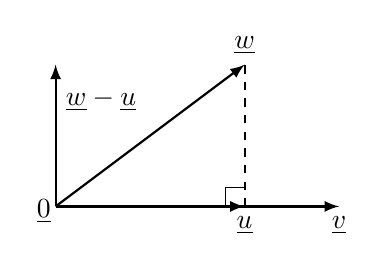
\begin{tikzpicture}[scale=0.6]
  \coordinate (v1) at (0,0);
  \coordinate (v2) at (4,3);
  \coordinate (v3) at (6,0);
  \coordinate (v4) at (4,0);
  \coordinate (v5) at (0,3);
  \path[draw] (3.6,0) -- (3.6,0.4) -- (4,0.4);
  \node (v0) at (-0.25,-0.1) {$\vecnot{0}$};
  \draw[-latex,thick] (v1) -- node[at end,above] {$\vecnot{w}$} (v2);
  \draw[-latex,thick] (v1) -- node[at end,below] {$\vecnot{v}$} (v3);
  \draw[-latex,thick] (v1) -- node[at end, below] {$\vecnot{u}$} (v4);
  \draw[thick,dashed] (v4) --  (v2);
  \draw[-latex,thick] (v1) -- node[right,near end] {$\vecnot{w}-\vecnot{u}$} (v5);
\end{tikzpicture}
\end{tabular}
\end{definition}

\end{frame}

\begin{frame}{3.6.1: Projection Lemma}

\begin{lemma}
Let $\vecnot{u}$ be the projection of $\vecnot{w}$ onto $\vecnot{v}$.
Then, $\langle \vecnot{w}-\vecnot{u} | \vecnot{u} \rangle = 0$ and \vspace{-1mm}
\[ \|\vecnot{w}-\vecnot{u}\|^2 =  \|\vecnot{w}\|^2 - \| \vecnot{u} \|^2 = \|\vecnot{w}\|^2 - \frac{|\langle \vecnot{w} | \vecnot{v} \rangle|^2}{\|\vecnot{v}\|^2}. \]
\end{lemma}
\begin{proof}
First, we observe that \vspace{-1mm}
\[ \langle \vecnot{w} - \vecnot{u} | \vecnot{v} \rangle = \langle \vecnot{w} | \vecnot{v} \rangle - \langle \vecnot{u} | \vecnot{v} \rangle = \langle \vecnot{w} | \vecnot{v} \rangle - \frac{\left\langle \vecnot{w} | \vecnot{v} \right\rangle}{\|\vecnot{v}\|^2} \langle \vecnot{v} | \vecnot{v} \rangle = 0. \vspace{-1.5mm} \]
Since $\vecnot{u} = s \vecnot{v}$ for some scalar $s$, it follows that $\langle \vecnot{w}-\vecnot{u} | \vecnot{u} \rangle =  0$.
Using $\langle \vecnot{w}-\vecnot{u} | \vecnot{u} \rangle = 0$, we can write \vspace{-1mm}
\begin{align*}
\|\vecnot{w}\|^2 &= \|(\vecnot{w}-\vecnot{u})+\vecnot{u}\|^2
= \langle (\vecnot{w}-\vecnot{u})+\vecnot{u}|(\vecnot{w}-\vecnot{u})+\vecnot{u}\rangle \\
&= \|\vecnot{w}-\vecnot{u}\|^2 + 2 \Real \langle \vecnot{w}-\vecnot{u} | \vecnot{u} \rangle + \|\vecnot{u}\|^2
= \|\vecnot{w}-\vecnot{u}\|^2 + \|\vecnot{u}\|^2. \vspace{-1mm}
\end{align*}
The proof is completed by noting that $\|\vecnot{u}\|^2 = |\langle \vecnot{w} | \vecnot{v} \rangle|^2 / \|\vecnot{v}\|^2$.
\end{proof}

\end{frame}

\begin{frame}{3.6.1: Properties of the Induced Norm}

\begin{theorem}
If $V$ is an inner-product space over $F$ and $\| \vecnot{v} \| \triangleq \sqrt{\left\langle \vecnot{v} | \vecnot{v} \right\rangle}$, then for any $\vecnot{v}, \vecnot{w} \in V$ and any $s\in F$, it follows that
\begin{enumerate}
\item $\left\| s \vecnot{v} \right\| = |s| \left\| \vecnot{v} \right\|$
\item $\left\| \vecnot{v} \right\| > 0$ for $\vecnot{v} \neq \vecnot{0}$
\item $\left| \left\langle \vecnot{v} | \vecnot{w} \right\rangle \right| \leq \left\| \vecnot{v} \right\| \left\| \vecnot{w} \right\|$ with equality iff $\vecnot{v} = \vecnot{0}$, $\vecnot{w}=\vecnot{0}$, or $\vecnot{v} = s \vecnot{w}$
\item $\left\| \vecnot{v} + \vecnot{w} \right\| \leq \left\| \vecnot{v} \right\| + \left\| \vecnot{w} \right\|$ with equality iff $\vecnot{v} = \vecnot{0}$, $\vecnot{w}=\vecnot{0}$, or $\vecnot{v} = s \vecnot{w}$.
\end{enumerate}
\end{theorem}

\begin{proof}[Sketch of Proof]<2->
The first two follow immediately from definitions.
The third inequality, $\left| \left\langle \vecnot{v} | \vecnot{w} \right\rangle \right| \leq \left\| \vecnot{v} \right\| \left\| \vecnot{w} \right\|$, is called the \textcolor{blue}{Cauchy-Schwarz inequality}.
The fourth inequality is the triangle inequality for the induced norm and can be shown using the Cauchy-Schwarz inequality.
\end{proof}

\visible<2->{Proof of Cauchy-Schwarz on whiteboard.}

\end{frame}

\begin{frame}{3.7: Sets of Orthogonal Vectors}

\begin{definition}<1->
Let $V$ be an inner-product space and $U,W$ be subspaces.
Then, the subspace $U$ is an \textcolor{blue}{orthogonal} to the subspace $W$ (denoted $U \bot W$) if: \vspace{-1.5mm}
$$ \vecnot{u} \ \bot \, \vecnot{w} \text{  for all } \vecnot{u}\in U \text{ and } \vecnot{w}\in W. $$
\end{definition}

\begin{definition}<2->
A subset $W\subset V$ of vectors is an \textcolor{blue}{orthogonal set} if all distinct pairs in $W$ are orthogonal.
A orthogonal set is \textcolor{blue}{orthonormal} if all vectors normalized.
\end{definition}

\begin{example}<3->
For $\RealNumbers^n$ with standard inner product, the standard basis is an orthonormal.
\end{example}

\begin{example}<4->
Let $V$ be the vector space (over $\ComplexNumbers$) of continuous functions $f\colon [0,1]\to\mathbb{C}$ with the standard inner product.
Let $f_n(x) = \sqrt{2} \cos 2 \pi n x$ and $g_n (x) = \sqrt{2} \sin 2 \pi n x$.
Then, $\{ 1, f_1, g_1, f_2, g_2, \ldots \}$ is a countably infinite orthonormal set and a Schauder basis for the closure of $V$.
\end{example}

\end{frame}

\begin{frame}{3.7: Properties of Orthogonal Sets}

\begin{lemma}<1->
Let $V$ be an inner-product space and $W\subset V$ be an orthogonal set of non-zero vectors.
Let $\vecnot{v} = s_1 \vecnot{w}_1 + \cdots + s_n \vecnot{w}_n$ be a linear combination of distinct vectors in $W$.
Then, \vspace{-2mm}
\[ s_i = \frac{ \left\langle \vecnot{v} | \vecnot{w}_i \right\rangle }
{ \left\| \vecnot{w}_i \right\|^2 }\]
\end{lemma}

\begin{proof}<2->
The inner product $\left\langle \vecnot{v} | \vecnot{w}_i \right\rangle$ is given by \vspace{-1mm}
\begin{equation*}
\begin{split}
\left\langle \vecnot{v} | \vecnot{w}_i \right\rangle
&= \left\langle \textstyle\sum_j s_j \vecnot{w}_j | \vecnot{w}_i \right\rangle
= \textstyle\sum_j s_j \left\langle \vecnot{w}_j | \vecnot{w}_i \right\rangle
= s_i \left\langle \vecnot{w}_i | \vecnot{w}_i \right\rangle .
\end{split} \vspace{-1mm}
\end{equation*}
Dividing both sides by $\| \vecnot{w}_i \|^2 = \left\langle \vecnot{w}_i | \vecnot{w}_i \right\rangle > 0$, gives the stated result.
\end{proof}

\begin{theorem}<3->
An orthogonal set of non-zero vectors is linearly independent.
\end{theorem}

\visible<3->{Proof by contradiction on whiteboard.}

\end{frame}

\begin{frame}{3.7: Unitary Matrices}

\begin{definition}
A complex matrix $U\in \ComplexNumbers^{n\times n}$ is called \textcolor{blue}{unitary} if $U^H U = I$.
Similarly, a real matrix $Q\in \RealNumbers^{n\times n}$ is called \textcolor{blue}{orthogonal} if $Q^T Q = I$.
\end{definition}

\begin{theorem}
Let $V = \ComplexNumbers^n$ be the standard inner product space and let  $U\in \ComplexNumbers^{n\times n}$ define a linear operator on $V$.
Then, the following conditions are equivalent:
\begin{enumerate}
\item[(i)] The columns of $U$ form an orthonormal basis (i.e.,  $U^H U = I$),
\item[(ii)] the rows of $U$ form an orthonormal basis (i.e.,  $U U^H = I$),
\item[(iii)] $U$ preserves inner products (i.e., $\langle U \vecnot{v} | U \vecnot{w} \rangle = \langle \vecnot{v} | \vecnot{w} \rangle$ for all $\vecnot{u},\vecnot{v}\in V$),
\item[(iv)] $U$ is an isometry (i.e., $\| U \vecnot{v} \| = \| \vecnot{v}\|$ for all $\vecnot{v} \in V$).
\end{enumerate}
\end{theorem}
\begin{proof}<2->
{\it(i)}$\Rightarrow${\it(ii)}: Orthogonal columns implies $U$ invertible and $U^H U = I$ implies $U^H = U^{-1}$.
{\it(i)}$\Rightarrow${\it(iii)}: $\langle U \vecnot{v} | U \vecnot{w} \rangle = \vecnot{w}^H U^H U \vecnot{v} = \vecnot{w}^H \vecnot{v} = \langle \vecnot{v} | \vecnot{w} \rangle$ and $\vecnot{w}=\vecnot{v}$ gives {\it(iv)}.
{\it(iv)}$\Rightarrow${\it(i)}:
$\vecnot{v}^H (U^H U \!-\! I) \vecnot{v} \!=\! \| U \vecnot{v} \|^2 \!-\! \| \vecnot{v} \|^2 \!=\! 0$
%because $\| U \vecnot{v} \| \!=\! \| \vecnot{v}\|$
and, as $U^H U \!-\! I$ is Hermitian, all eigenvalues are 0 and $U^H U - I = 0$.
\end{proof}

\end{frame}

\begin{frame}{3.7: Gram-Schmidt Orthogonalization (1)}

\begin{block}{Gram-Schmidt Process}
Let $V$ be an inner-product space and assume $\vecnot{v}_1, \ldots, \vecnot{v}_n$ are linearly independent vectors in $V$.
Then, an orthogonal set of vectors $\vecnot{w}_1, \ldots, \vecnot{w}_n$ with the same span is produced by \textcolor{blue}{Gram-Schmidt process}:
\begin{enumerate}
\item Let $\vecnot{w}_1 = \vecnot{v}_1$

\item For $m=1,\ldots,n-1$, define \vspace{-3.5mm}
\begin{equation*}
\vecnot{w}_{m+1} = \vecnot{v}_{m+1} - \sum_{i=1}^m \frac{ \left\langle \vecnot{v}_{m+1} | \vecnot{w}_i \right\rangle } { \left\| \vecnot{w}_i \right\|^2 } \vecnot{w}_i.
\end{equation*}
\end{enumerate}
\end{block}

\begin{itemize}
\item<2-> Vector $\vecnot{w}_{m+1} \neq 0$. Otherwise, $\vecnot{v}_{m+1}$ is a linear combination of $\vecnot{w}_1, \ldots, \vecnot{w}_m$ and hence a linear combination of $\vecnot{v}_1, \ldots, \vecnot{v}_m$ \vspace{2.5mm}

\item<3-> Vectors $\vecnot{w}_{m+1}$ and $\vecnot{w}_j$ are orthogonal for $j=1,\ldots,m$: \vspace{-1.5mm}
\begin{equation*}
\begin{split}
\left\langle \vecnot{w}_{m+1} | \vecnot{w}_j \right\rangle
&= \left\langle \vecnot{v}_{m+1} | \vecnot{w}_j \right\rangle
- \sum_{i=1}^m \frac{ \left\langle \vecnot{v}_{m+1} | \vecnot{w}_i \right\rangle } { \left\| \vecnot{w}_i \right\|^2 }
\left\langle \vecnot{w}_i | \vecnot{w}_j \right\rangle \\
&= \left\langle \vecnot{v}_{m+1} | \vecnot{w}_j \right\rangle
- \frac{ \left\langle \vecnot{v}_{m+1} | \vecnot{w}_j \right\rangle } { \left\| \vecnot{w}_j \right\|^2 }
\left\langle \vecnot{w}_j | \vecnot{w}_j \right\rangle = 0
\end{split}
\end{equation*}

\end{itemize}

\end{frame}

\begin{frame}{3.7: Gram-Schmidt Orthogonalization (2)}

\begin{example}
Let $V = \RealNumbers^3$ be standard vector space equipped with the standard inner product and define \vspace{-4mm}
\begin{align*}
\vecnot{v}_1 &= (2,2,1) \\
\vecnot{v}_2 &= (3,6,0) \\
\vecnot{v}_3 &= (6,3,9)
\end{align*}
\vspace{-4mm}

Applying the Gram-Schmidt process to $\vecnot{v}_1, \vecnot{v}_2, \vecnot{v}_3$ results in: \vspace{-2mm}
\begin{align*}
\visible<1->{\vecnot{w}_1 &= \textcolor{blue}{(2,2,1)} \\}
\visible<2->{\vecnot{w}_2 &= (3,6,0)
- \frac{ \left\langle (3,6,0) | (2,2,1) \right\rangle }{ 9 } (2,2,1) \\}
\visible<3->{&= (3,6,0) - 2 (2,2,1) = \textcolor{blue}{(-1,2,-2)} \\}
\visible<4->{\vecnot{w}_3 &= \vecnot{v}_3
- \frac{ \left\langle (6,3,9) | (2,2,1) \right\rangle }{ 9 } (2,2,1)
- \frac{ \left\langle (6,3,9) | (-1,2,-2) \right\rangle }{ 9 } (-1,2,-2) \\}
\visible<5->{&= (6,3,9) - 3 (2,2,1) + 2 (-1,2,-2) = \textcolor{blue}{(-2,1,2)}}
\end{align*}
\visible<6->{It is easily verified that $\{ \vecnot{w}_1, \vecnot{w}_2, \vecnot{w}_3\}$ is an orthogonal set of vectors.}
\end{example}

\end{frame}

\begin{frame}{3.7.1: Hilbert Spaces}

\begin{definition}
A complete inner-product space is called a \textcolor{blue}{Hilbert space}.
\end{definition}

\begin{example}
Consider the Banach space $\ell^2$ of infinite real/complex sequences with Euclidean norm $\|\vecnot{v}\| = \left( \sum_{i=1}^\infty |v_i|^2 \right)^{1/2} < \infty$.
The set $\ell^2$ is a Hilbert space under the standard inner product because it induces the Euclidean norm.
\end{example}

\begin{theorem} 
If Hilbert space $V$ has a countable dense subset, then there is a linear transform $T:V\to \ell^2$ such that $\left\langle \vecnot{u} | \vecnot{v} \right\rangle_V = \left\langle T\vecnot{u} | T\vecnot{v} \right\rangle_{\ell^2}$ for all $\vecnot{u},\vecnot{v} \in V$.
\end{theorem}

%\begin{example}[Quantum Mechanics]
%Quantum mechanics is derived in the Hilbert space $\ell^2$ because:
%\begin{itemize}
%\item the state of a closed $n$-dimensional quantum systems is modeled by a unit vector in the standard inner product space for $\mathbb{C}^n$
%\item all allowable operations on the system result either in unitary evolution or a known projection of that vector
%\item sequentially joining the states of all quantum systems in the universe gives a sequence of state vectors of dimension tending to infinity
%\end{itemize}
%\end{example}

\end{frame}

%\begin{frame}{3.7: Orthogonal Complement}
%
%\begin{definition}
%Let $V$ be an inner-product space and $W$ be any set of vectors in $V$.
%The \textcolor{blue}{orthogonal complement} of $W$ denoted by $W^{\bot}$ is the set of all vectors in $V$ that are orthogonal to every vector in $W$ or
%\begin{equation*}
%W^{\bot} = \left\{ \vecnot{v} \in V \big| \langle \vecnot{v} | \vecnot{w} \rangle = 0 \; \forall \; \vecnot{w}\in W \right\}. 
%\end{equation*}
%\end{definition}
%
%\end{frame}

\begin{frame}{3.8: Linear Functionals and the Riesz Theorem}

\begin{definition}
Let $V$ be a vector space over a field $F$.
A linear transformation $f$ from $V$ into the scalar field $F$ is called a \textcolor{blue}{linear functional} on $V$.
\end{definition}

\begin{example}
Thus, $f\colon V \to F$ is a function on $V$ such that
\begin{equation*}
f \left( s \vecnot{v}_1 + \vecnot{v}_2 \right)
= s f \left( \vecnot{v}_1 \right) + f \left( \vecnot{v}_2 \right)
\end{equation*}
for all $\vecnot{v}_1, \vecnot{v}_2 \in V$ and $s \in F$.
\end{example}

\begin{theorem}[Riesz]
Let $V$ be a Hilbert space and $f$ be a continuous linear functional on $V$.
Then, there exists a unique vector $\vecnot{v} \in V$ such that $f \left( \vecnot{w} \right) = \left\langle \vecnot{w} | \vecnot{v} \right\rangle$ for all $\vecnot{w} \in V$.
\end{theorem}

\end{frame}

\begin{frame}{Derivatives in Banach Spaces}

The foundation of engineering is the ability to use math and physics to design and optimize complex systems.

\vspace{3mm}

Computers have now made this possible on an unprecedented scale.

\vspace{3mm}

In vector analysis, derivatives are usually introduced using Banach spaces: \vspace{-2mm}
\begin{itemize}
\item<1-> For a function $f \colon X \rightarrow Y$, the definition of the derivative requires a linear structure (to define differences) and a topology (to define convergence) on both $X$ and $Y$ \vspace{1mm}

\item<2-> If $X=\RealNumbers^n$ and $Y=\RealNumbers^m$, then the derivative is a linear transform from $X$ to $Y$ represented by the Jacobian matrix $f'(\vecnot{x}) \in \RealNumbers^{m\times n}$ \vspace{1mm}

\item<3-> Thus, we generally assume $f \colon X \rightarrow Y$ be a mapping from the Banach space $(X,\|\cdot\|_X)$ to the Banach space $(Y,\|\cdot\|_Y)$ \vspace{1mm}

\item<4-> For directional derivatives, one only needs the linear structure on $X$
\end{itemize}
\end{frame}

\begin{frame}{Directional Derivatives}

\begin{definition}[Directional Derivative]<1->
Let $f \colon X \rightarrow Y$ map vector space $X$ to a Banach space $(Y,\|\cdot\|)$.
Then, if it exists, the \textcolor{blue}{G\^{a}teaux differential} of $f$ at  $\vecnot{x}$ in direction $\vecnot{h}$ is given by \vspace{-1.5mm}
\[ \delta f (\vecnot{x};\vecnot{h}) \triangleq \lim_{t \to 0} \frac{f(\vecnot{x}+t \vecnot{h}) - f(\vecnot{x})}{t}. \]
%where the limit is with respect to the implied mapping from $\RealNumbers$ to $Y$.
\end{definition}

\begin{example}<2->
Consider $X\!=\!Y\!=\!\mathbb{R}^2$ and $f(\vecnot{x})\! =\! (x_1 x_2,x_1+x_2^2)$.
For $\vecnot{x}\!=\!(1,1)$, $\vecnot{h}\!=\!(1,2)$: \vspace{-2.5mm}
\[ \delta f ( \vecnot{x},\vecnot{h} ) = \frac{d}{dt} ((1+t)(1+2t),(1+t)+(1+2t)^2) \Big|_{t=0} = (3,5). \]
\end{example}

\begin{lemma}<3->
Let $Y=\RealNumbers$ and suppose that $\delta f (\vecnot{x};\vecnot{h})$ exists and is negative for some $f$, $\vecnot{x}$, and $\vecnot{h}$.  Then, there exists $t_0 > 0$ such that, for all $t\in(0,t_0)$, one has \vspace{-2mm}
\[ f(\vecnot{x}+t \vecnot{h}) < f (\vecnot{x}). \]
\end{lemma}

\visible<3->{Proof on whiteboard.}

\end{frame}

\begin{frame}{What is Meant by Differentiable?}

\begin{definition}
Let $f \colon X \rightarrow Y$ be a mapping from a vector space $X$ to a Banach space $(Y,\|\cdot\|)$.
Then, $f$ is \textcolor{blue}{G\^{a}teaux differentiable} at $\vecnot{x}$ if the G\^{a}teaux differential $\delta f (\vecnot{x};\vecnot{h})$ exists for all $\vecnot{h} \in X$ and is a continuous linear function of $\vecnot{h}$.
\end{definition}

\begin{definition}[Differentiable]
Let $f \colon X \rightarrow Y$ be a mapping from a Banach space $(X,\|\cdot\|_X)$ to a Banach space $(Y,\|\cdot\|_Y)$.
Then, $f$ is \textcolor{blue}{Fr\'{e}chet differentiable} at $\vecnot{x}$ if there is a continuous linear transformation $T\colon X \to Y$ satisfying
\begin{equation*} \lim_{\vecnot{h} \to \vecnot{0}} \frac{\left\|f(\vecnot{x}+ \vecnot{h}) - f(\vecnot{x}) - T(\vecnot{h}) \right\|_Y}{\| \vecnot{h} \|_X} = 0,
\end{equation*}
where the limit is with respect to the implied Banach space mapping $X\to \RealNumbers$.
In this case, the \textcolor{blue}{Fr\'{e}chet derivative} $f'(\vecnot{x})$ equals $T$.
\end{definition}
\end{frame}

\begin{frame}{Gradient Descent}

\begin{itemize}
\item<1-> Gradient descent subtracts the gradient $\nabla f(\vecnot{x})$ from an element of $X\!\!\!$ \vspace{1mm}

\item<2-> But, for a Banach space, the derivative is a linear functional mapping $X$ to $\RealNumbers$!

\item<3-> How can one add a linear mapping to $X$?

\item<4-> In Hilbert space, the Riesz representation theorem states every linear functional is represented by the inner product with a fixed vector

\item<5-> Thus, the gradient $\nabla f (\vecnot{x}) \in X$ is defined as the representative vector
\end{itemize}

\begin{definition}[Gradient Descent]<6->
Let $f \colon X \rightarrow \RealNumbers$ be a mapping from a Hilbert space $X$ to the standard Banach space of real numbers.
Starting from $\vecnot{x}_1 \in X$, \textcolor{blue}{gradient descent} defines the sequence \vspace{-4mm}
\[ \vecnot{x}_{n+1} = \vecnot{x}_n - \delta_n \nabla f(\vecnot{x}_n), \]
where $\delta_n$ is the step size and the gradient $\nabla f (\vecnot{x})$ is uniquely defined by \vspace{-1.5mm}
\[\langle \vecnot{h} | \nabla f(\vecnot{x}) \rangle = f'(\vecnot{x})(\vecnot{h}) \text{ for all } \vecnot{h} \in X. \]
\end{definition}


\end{frame}


\backupbegin

%\begin{frame}
%\frametitle{Backup Slides}
%\begin{itemize}
%\item Slide numbers not included in denominator!
%\end{itemize}
%\end{frame}

%\begin{frame}[allowframebreaks]
%\frametitle{References}
%\bibliographystyle{alpha}
%\footnotesize
%\bibliography{IEEEabrv,WCLabrv,WCLbib,WCLnewbib}
%\end{frame}

\backupend

\end{document}
